\documentclass[11pt]{article}
\usepackage{UF_FRED_paper_style}

\usepackage[utf8]{inputenc}
\usepackage[T1]{fontenc}
\usepackage[english]{babel}
\usepackage{microtype} % optional, for aesthetics
\usepackage{tabularx} % nice to have
\usepackage{booktabs} % necessary for style
% \usepackage{graphicx}
% \graphicspath{{./figures/}}
% \usepackage{listings}
% \lstset{...}

% \newcommand\code[1]{\texttt{#1}}
% \let\file\code
\usepackage{listings}
\usepackage{color}

\definecolor{dkgreen}{rgb}{0,0.6,0}
\definecolor{gray}{rgb}{0.5,0.5,0.5}
\definecolor{mauve}{rgb}{0.58,0,0.82}

\lstset{frame=tb,
  language=c,
  aboveskip=3mm,
  belowskip=3mm,
  showstringspaces=false,
  columns=flexible,
  basicstyle={\small\ttfamily},
  numbers=none,
  numberstyle=\tiny\color{gray},
  keywordstyle=\color{blue},
  commentstyle=\color{dkgreen},
  stringstyle=\color{mauve},
  breaklines=true,
  breakatwhitespace=true,
  tabsize=3
}

\onehalfspacing

\setlength{\droptitle}{-5em} %% Don't touch

% TITLE:
\title{Batalha Naval Cliente Servidor TCP}
\author {Lucca Augusto}

% DATE:
\date{\today}

\begin{document}

\maketitle

\section{Descrição}
Trabalho desenvolvido para a disciplina de redes do primeiro semestre de 2020.
Este trabalho consistem em um jogo de batalha naval entre cliente e servidor utilizando a biblioteca socket e o padrão TCP.
O jogo ocorre em turnos, primeiro o cliente ataca, depois o servidor, até que algum dos dois perca.
O programa foi implementado em C e usa a biblioteca sys/socket. 

\section{Compilação e execução}
O programa é compilado pelo makefile usando o comando

\begin{lstlisting}
make
\end{lstlisting}

Para executar o programa é preciso executar primeiro o servidor e depois o cliente, já que o cliente nao conseguirá se conectar se o servidor nao estiver rodando.
Utilizando o comando seguinte é possível executar o programa em apenas uma instância do shell. Executa o servidor em background e o cliente em seguida.

\begin{lstlisting}
./servidor [-p porta] &
./cliente [-i ip] [-p porta] [-a arquivo]
\end{lstlisting}

Uma outra forma de executar é usar um shell para o servidor e um shell para o cliente.

(shell 1)
\begin{lstlisting}
./servidor [-p porta]
\end{lstlisting}


(shell 2)
\begin{lstlisting}
./cliente [-i ip] [-p porta] [-a arquivo]
\end{lstlisting}

Caso nenhum argumento seja passado aos programas, o servidor iniciará na porta padrão 8000, o cliente acessará a porta padrao 8000 com o ip padrao 127.0.0.1 e carregara o tabuleiro do arquivo tabuleiro.txt

O arquivo de configuração do tabuleiro deve ser um arquivo texto no seguinte formato:
Cada linha representa um navio, a linha deve começar com 2 letras que indicam qual navio a linha representa. pa para Porta-Avião, nt para Navio-Tanque, ct para Contratorpedeiro e sb para submarino. Depois dessa informação vem as coordenadas mais a esquerda e a cima do navio, o ponto inicial do navio, separadas por espaços. Em seguida vem a letra 'v' ou 'h', indicando se o navio está na vertical ou horizontal respectivamente. 

\section{Código}
O código é composto por 4 arquivos:
\begin{itemize}
\item servidor.c
\item cliente.c
\item batnaval.h
\item utils.h
\end{itemize}

\subsection{servidor.c}
O arquivo servidor.c é responsável por inicializar o socket e ouvir a porta.
Após inicializar o socket, o servidor fica em espera até algum cliente se conectar na porta.
Feita a conexão, o servidor espera pela mensagem do cliente com as coordenadas de seu ataque.
O servidor executa um loop até que receba do cliente a mensagem "perdi", informando que o cliente perdeu, ou até que o servidor perca o jogo, enviando para o cliente a mensagem "perdi" e finalizando sua execução.
Recebida a mensagem de ataque, o ataque é computado e o servidor devolve uma mensagem para o cliente.
Essa mensagem é da forma "x y 1" onde x e y sao as coordenadas do ataque gerado pelo servidor e 1 é uma flag
dizendo se o ataque anterior do cliente acertou algum navio.
\subsubsection{Ataque do servidor}
O ataque do servidor acontece da seguinte forma: Chuta uma coordenada aleatória na primeira vez, se acertar algum navio, or próximos ataques acontecem nas coordenadas adjacentes ao ponto acertado.
\subsubsection{Recebendo um ataque do cliente}
Caso a mensagem do cliente não seja "perdi", o servidor computa o ataque marcando um 0 em seu tabuleiro nas coordenadas informadas pelo jogador.

\subsection{cliente.c}
O arquivo cliente.c é responsavel por se conectar a porta e realizar os ataques indicados pelo usuário.
Após inicializar o socket, o cliente conecta na porta e espera pela entrada do usuário com as coordenadas de seu ataque.
Após o usuário digitar as coordenadas, o cliente envia para o servidor uma mensagem com as coordenadas do ataque na forma "x y 1" onde x e y são a linha e a coluna do ataque, respectivamente, e 1 é uma flag que indica se o último ataque do servidor acertou.
Depois disso o cliente executa um loop até receber do servidor a mensagem "perdi" informando que o servidor perdeu, ou até que o cliente perca o jogo, enviando para o servidor a mensagem "perdi" e finalizando sua execução.

\subsubsection{Ataque do cliente}
O usuário digita as coordenadas de seu ataque, linha (em número) e coluna (em letra) e o cliente monta a mensagem e envia ao servidor. Caso o usuário digite 'p' ao informar a linha, o cliente mostrará na tela a disposição de seu tabuleiro e um mapa de seus acertos no tabuleiro inimigo.

\subsubsection{Recebendo um ataque do servidor}
Caso a mensagem enviada pelo servidor não seja "perdi", o cliente computa o ataque marcando um 0 em seu tabuleiro nas coordenadas enviadas pelo servidor.

\subsection{utils.h}
Esse arquivo contém funções de IO e utéis para todos os arquivos em geral.

\subsection{batnaval.h}
Esse arquivo implementa o jogo de batalha naval em sí. Ele é responsável por computar as jogadas, verificar se o dono do tabuleiro atual perdeu e inicializar os tabuleiros, lendo de um arquivo ou gerando aleatóriamente.

\section{Screenshots}

\begin{figure}[H]
    \centering
        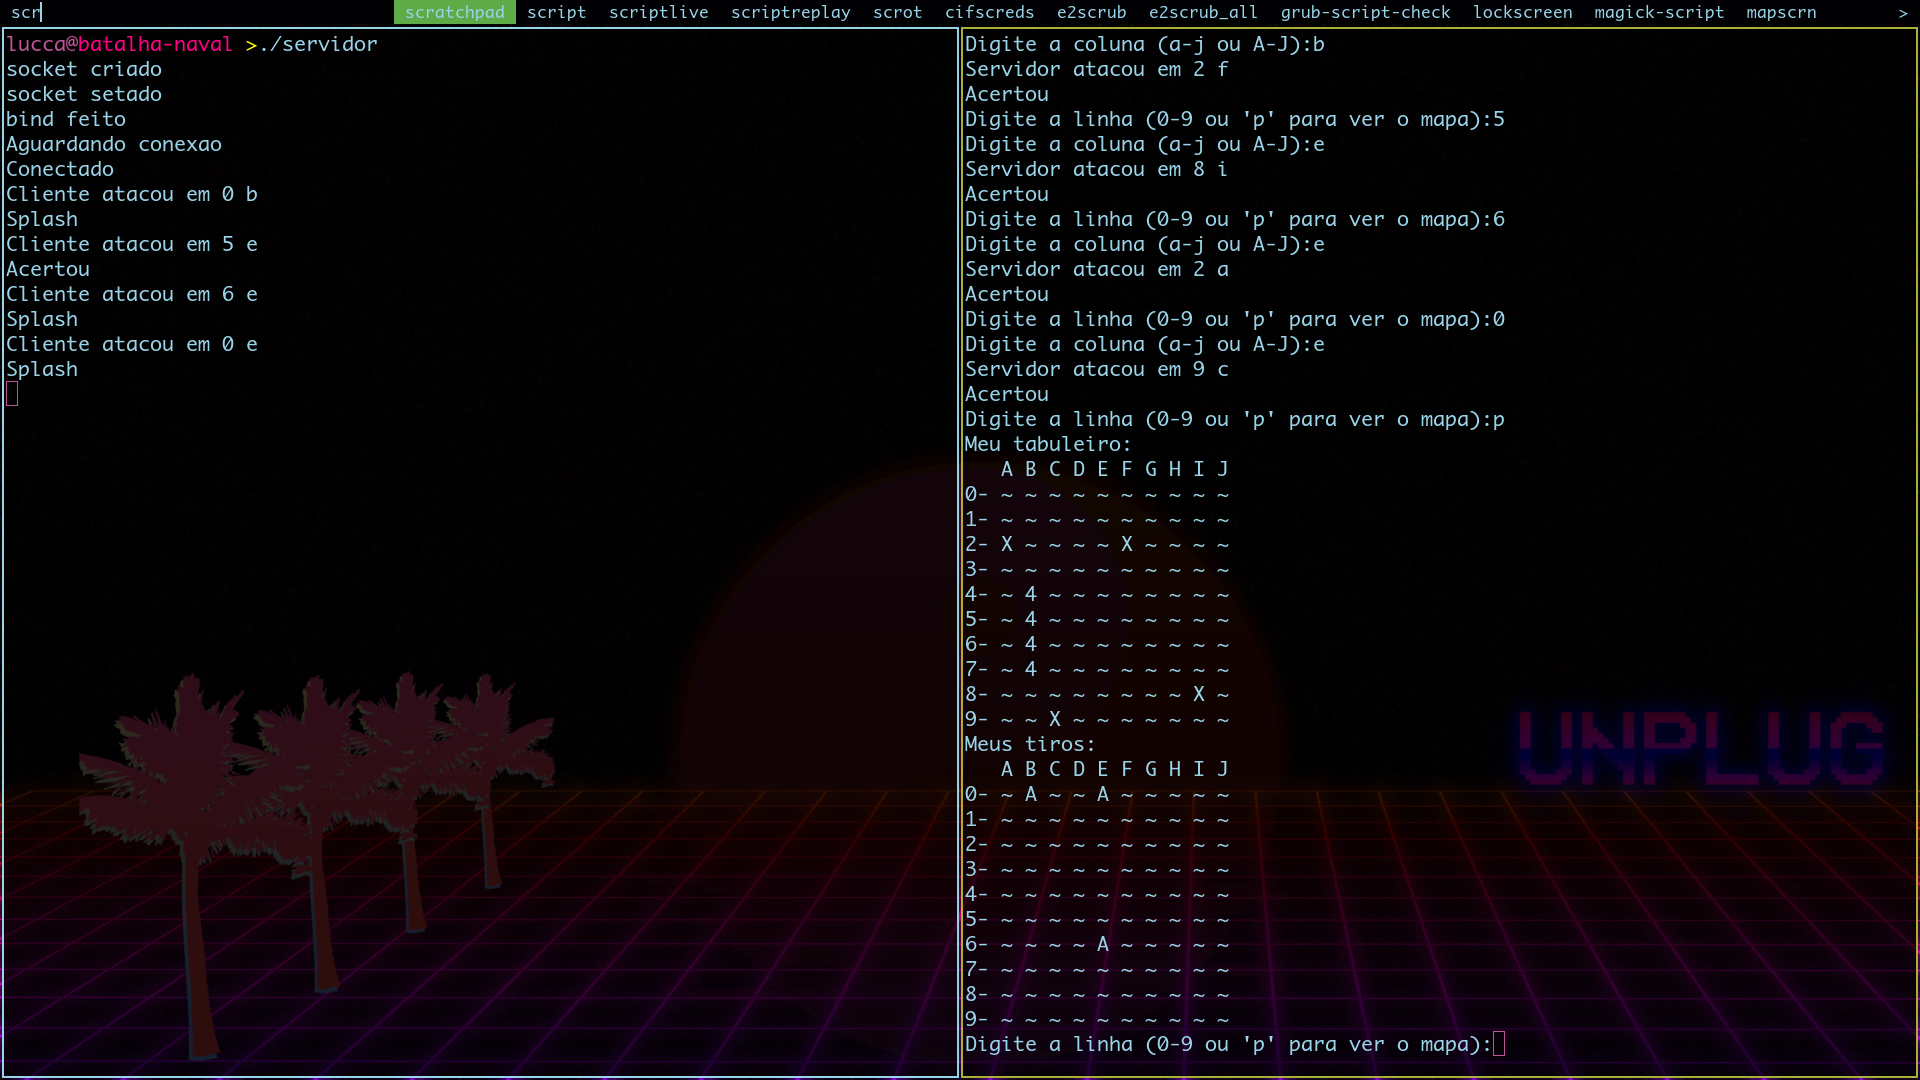
\includegraphics[scale=.2]{scrot_batnaval.png}
    \caption{Screenshot mostrando a execução do programa}
    \label{fig:1}
\end{figure}
\end{document}
